\section{Overview}
% BDD Generelt:
% - Feature

In order to pursue the goal of introducing contracts to BDD and easing the continued work on a given software development project, we introduce The Salad Framework. Salad contains three DSLs --- each with a specific purpose. Gherkin is the BDD feature specification language, Lettuce is the transformation language and lastly, Tomato is a simplified version of JML.  Combined, they make it possible for contracts to be extracted and generated from feature descriptions and transformed into JML. Figure \ref{fig:saladoverview} presents the workflow from input to output.

\begin{figure}
	\begin{center}
		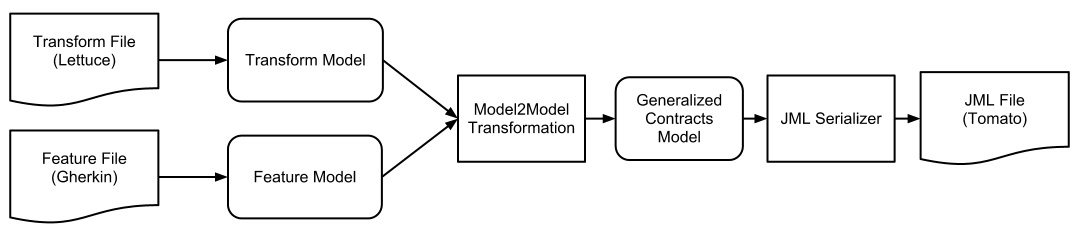
\includegraphics[scale=0.46]{images/framework_overview.png}
	\end{center}
	\caption{Salad Framework Overview}
	\label{fig:saladoverview}
\end{figure}

The Feature Model represents an extension of Cucumber feature language which is the main artifact in BDD. We want to allow people already familiar with BDD-features to work in an environment that they are accustomed to. This is achieved by extending the original, well-known feature language, instead of creating a new language. We want the extending parts of the feature language we introduce in this project to be done with as much respect to the original feature language's textual syntax as possible. The meta-model Having this rich model and language, that contains both the original features of the feature language as well as our extension, also allow for further development on the project as all elements of the language are available in the model. One could do a transformation to a simplified model accepted by standard BDD tools, which will allow the further generation of regular test-cases.

The Transform Model specifies how the contracts written in natural language in the feature file are transformed to actual contracts. By specifying rules on how contracts are interpreted, the user decides the nature of the language in which the natural language contracts are represented. 

Through model-to-model transformation the feature model(s) and the transform model(s) are transformed into a meta-model representing a subset of JML, namely code contracts describing pre- and postconditions. The textual representation of our JML model resembles Java syntax with classes containing methods and their contracts written in JML.
